\chapter{Fundamentos teóricos}
\label{cap:fundamentos_teoricos}
Este capítulo se enfoca en analizar en profundidad los aspectos técnicos necesarios para llevar a cabo el desarrollo del CanSat.
Se incluye una comparativa entre los distintos microcontroladores y microcomputadores disponibles en el mercado, evaluando su precio, disponibilidad y adecuación a los requisitos técnicos del proyecto.
Además, se analizan los sensores y módulos de comunicación más comunes, así como los principales protocolos utilizados para la comunicación entre el microcontrolador y los sensores, como I2C y UART.
También se estudian distintas opciones para la retransmisión de vídeo en tiempo real desde el CanSat.
Por último, se exploran soluciones para la visualización de los datos a través de una interfaz web en tiempo real.


\section{Comparativa de microcontroladores y microcomputadores}
Uno de los componentes principales de un CanSat o de cualquier sistema embebido en general es su microcontrolador o microcomputador,
es el encargado de comunicarse con los sensores, procesar los datos y transmitirlo a través del módulo de comunicación,
también es el encargado de procesar el video y retransmitirlo en tiempo real(si el hardware lo permite).

Primero conviene aclarar la diferencia entre microcontrolador y microcomputador:
\begin{itemize}
    \item \textbf{Microcontrolador:} Circuito integrado que combina procesador, memoria y periféricos de entrada/salida en un solo chip.
    Está diseñado para realizar tareas específicas con bajo consumo energético y recursos limitados.
    Es común en aplicaciones como lectura de sensores, control de motores o gestión de comunicaciones básicas.
    Ejemplos comunes son Arduino Uno o ESP32
    \item \textbf{Microcomputador:} Sistema completo en una sola placa (Single-Board Computer) que integra procesador, memoria, almacenamiento y puertos de expansión.
    Es capaz de ejecutar sistemas operativos completos (como Linux) y realizar tareas más complejas, como procesamiento de imágenes, servidor web o interfaces gráficas.
    Un ejemplo típico es la Raspberry Pi Zero.
\end{itemize}

Actualmente, en el mercado se pueden encontrar varios de estos microcontroladores o microcomputadores de bajo coste, tamaño y peso reducido y bajo consumo.
En esta sección nos vamos a centrar en el análisis de tres de las opciones más populares:
\begin{itemize}

    \item \textbf{\cite{raspberrypi_zero2}:}
    La Raspberry Pi Zero 2 es un Single Board Computer de bajo costo lanzado en Reino Unido por la~\cite{raspberrypi_foundation},
    de toda la familia Raspberry Pi se ha elegido el modelo Zero 2 por ser el de tamaño más reducido pero con una potencia adecuada para el desarrollo de un proyecto como el CanSat.
    Las características más relevantes para este proyecto son:
    \begin{itemize}
        \item CPU Arm Cortex-A53 de cuatro núcleos y 64 bits a 1 GHz.
        \item SDRAM de 512 MB.
        \item LAN inalámbrica de 2,4 GHz 802.11 b/g/n.
        \item Bluetooth 4.2, Bluetooth Low Energy (BLE), antena integrada.
        \item Ranura para tarjeta microSD.
        \item Conector de cámara CSI-2.
        \item Cabecera GPIO de 40 pines para conexión de periféricos.
        \item 1 × SPI
        \item 2 × interfaces I²C
        \item 1 × UART
        \item Consumo típico de energía: entre 0.7\,W y 1.5\,W dependiendo de la carga de trabajo.
        \item Precio aproximado: 15–20€.
    \end{itemize}
    \begin{figure}[h]
        \centering
        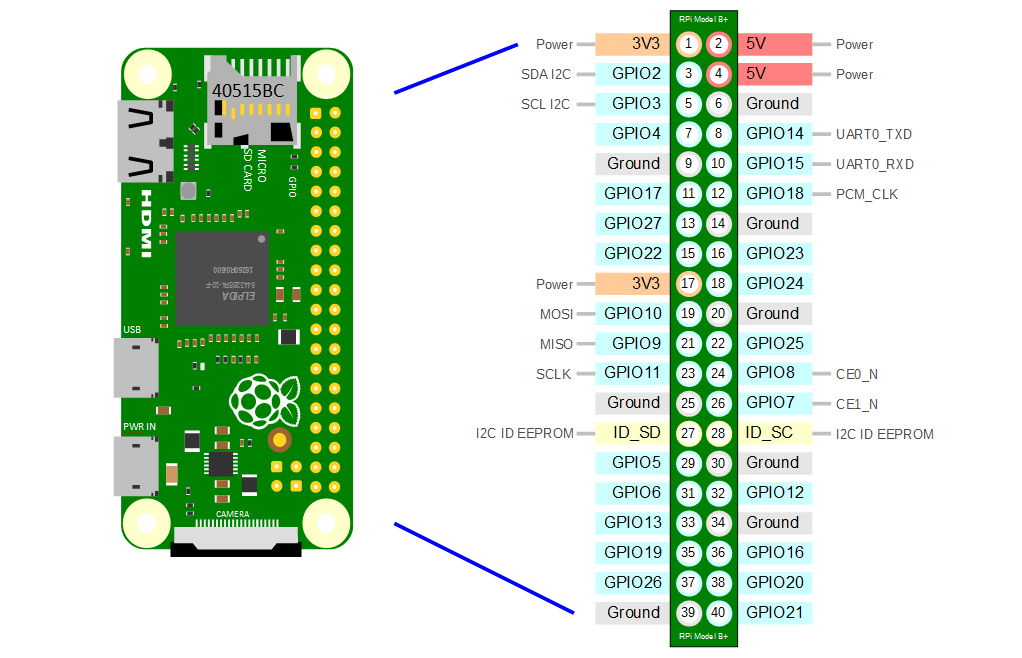
\includegraphics[width=0.8\textwidth]{Imagenes/Bitmap/pizero2gpio}
        \caption{Distribución de pines GPIO en Raspberry Pi Zero 2}
        \label{fig:pizer2_gpio}
    \end{figure}
    Como se puede ver en las características la Raspberry Pi Zero 2 cumple con los requisitos necesarios para este proyecto,
    cuenta con un procesador y memoria adecuados, soporte para cámara (útil para la retransmisión de video en tiempo real), conectividad inalámbrica mediante WiFi
    y compatibilidad con los protocolos I\textsuperscript{2}C y UART mediante los pines GPIO necesarios para la conexión directa de sensores.

    \item \textbf{\cite{esp32}:}
    Es un microcontrolador de bajo coste desarrollado por Espressif Systems que combina bajo coste con buena capacidad de procesamiento y conectividad inalámbrica integrada,
    lo que lo convierte en una de las opciones más populares para proyectos embebidos, incluyendo CanSat.

    A diferencia de un microcomputador como la Raspberry Pi, el ESP32 no ejecuta un sistema operativo generalista,
    pero su bajo consumo energético y la integración de múltiples periféricos lo hacen convierten en muy buena opción cuando se busca eficiencia y simplicidad del sistema.

    Las características más relevantes para este proyecto son:
    \begin{itemize}
        \item CPU dual-core Tensilica Xtensa LX6 a 240\,MHz.
        \item 520\,KB de SRAM interna.
        \item Memoria flash externa: normalmente 4\,MB (dependiendo del modelo).
        \item Conectividad Wi-Fi 802.11 b/g/n.
        \item Bluetooth 4.2 y BLE.
        \item 4 × SPI
        \item 2 × interfaces I²C
        \item 3 × UART
        \item Hasta 34 pines GPIO (según versión del módulo).
        \item Consumo típico: entre 0.2\,W y 0.6\,W, dependiendo del modo de operación.
        \item Precio aproximado: 4–8€~\cite{esp32}.
    \end{itemize}
    \begin{figure}[h]
        \centering
        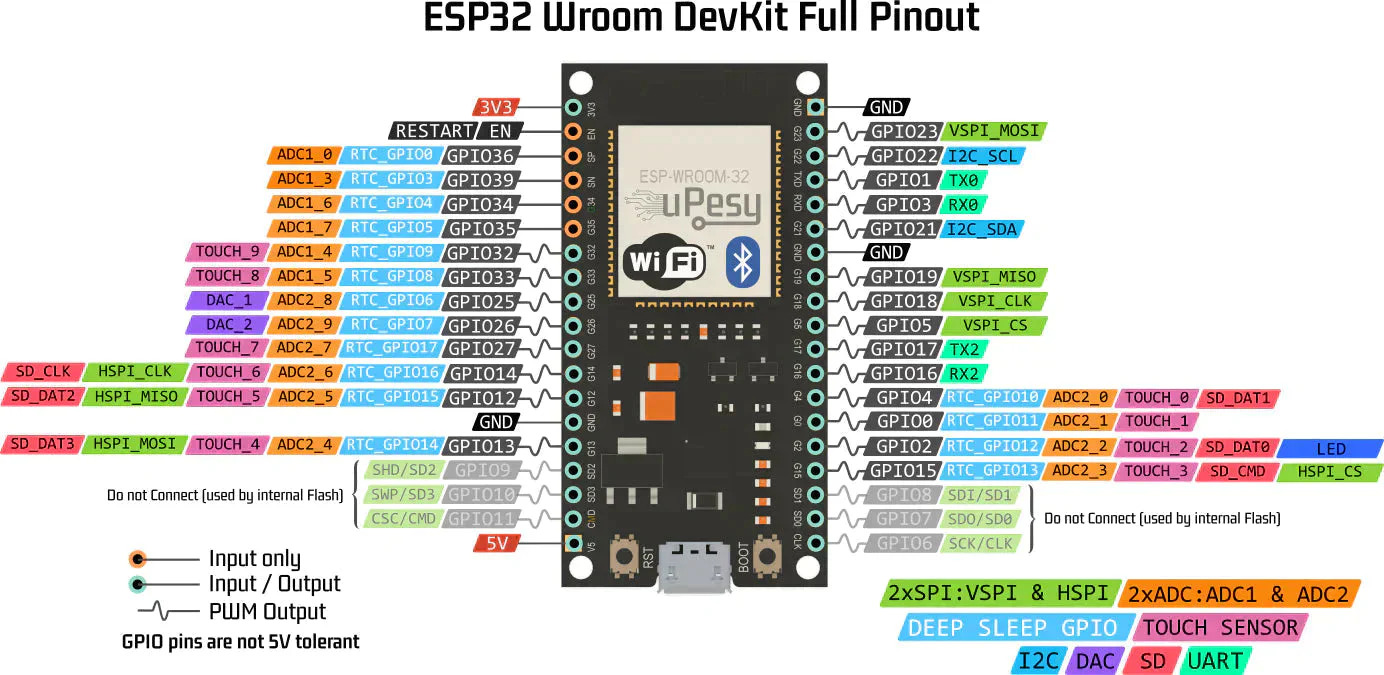
\includegraphics[width=0.8\textwidth]{Imagenes/Bitmap/esp32gpio}
        \caption{Distribución de pines GPIO en ESP32}
        \label{fig:esp32gpio}
    \end{figure}

    Gracias a su bajo consumo, potencia y multiples conexiones, el ESP32 permite integrar sensores fácilmente a través de interfaces estándar y puede encargarse tanto de la adquisición como de la transmisión de datos por radio o Wi-Fi.
    Además, su bajo consumo lo hace especialmente adecuado para sistemas alimentados por batería en entornos con restricciones energéticas.
    También existen variantes como el ESP32-CAM que integran una cámara de tipo OV2640, lo que permite capturar imágenes y transmitir video mediante Wi-Fi
    aunque con un rendimiento y resolución inferior a la de Raspberry Pi.

    \item \textbf{\cite{arduino_nano}:}
    Es un microcontrolador compacto de bajo coste basado en el chip ATmega328P, es el más utilizado en entornos educativos gracias a su simplicidad,
    por lo que cuenta con una amplia comunidad detrás y desarrollo de librerias.
    A diferencia de la Raspberry Pi Zero 2 o el ESP32, el Arduino Nano no cuenta con conectividad inalámbrica ni capacidad de procesamiento avanzada,
    pero es suficiente para gestionar sensores básicos y transmitir datos mediante un módulo externo de radio.

    Las características más relevantes para este proyecto son:
    \begin{itemize}
        \item Microcontrolador ATmega328P.
        \item Frecuencia de reloj: 16\,MHz.
        \item Memoria flash: 32\,KB (2\,KB utilizados por el bootloader).
        \item SRAM: 2\,KB.
        \item EEPROM: 1\,KB.
        \item 22 pines GPIO (14 digitales, 8 analógicos).
        \item 1 × interfaz I²C.
        \item 1 × UART.
        \item 1 × SPI.
        \item Consumo típico: entre 0.05\,W y 0.2\,W.
        \item Precio aproximado: 27€ en la web oficial.
    \end{itemize}

    \begin{figure}[H]
        \centering
        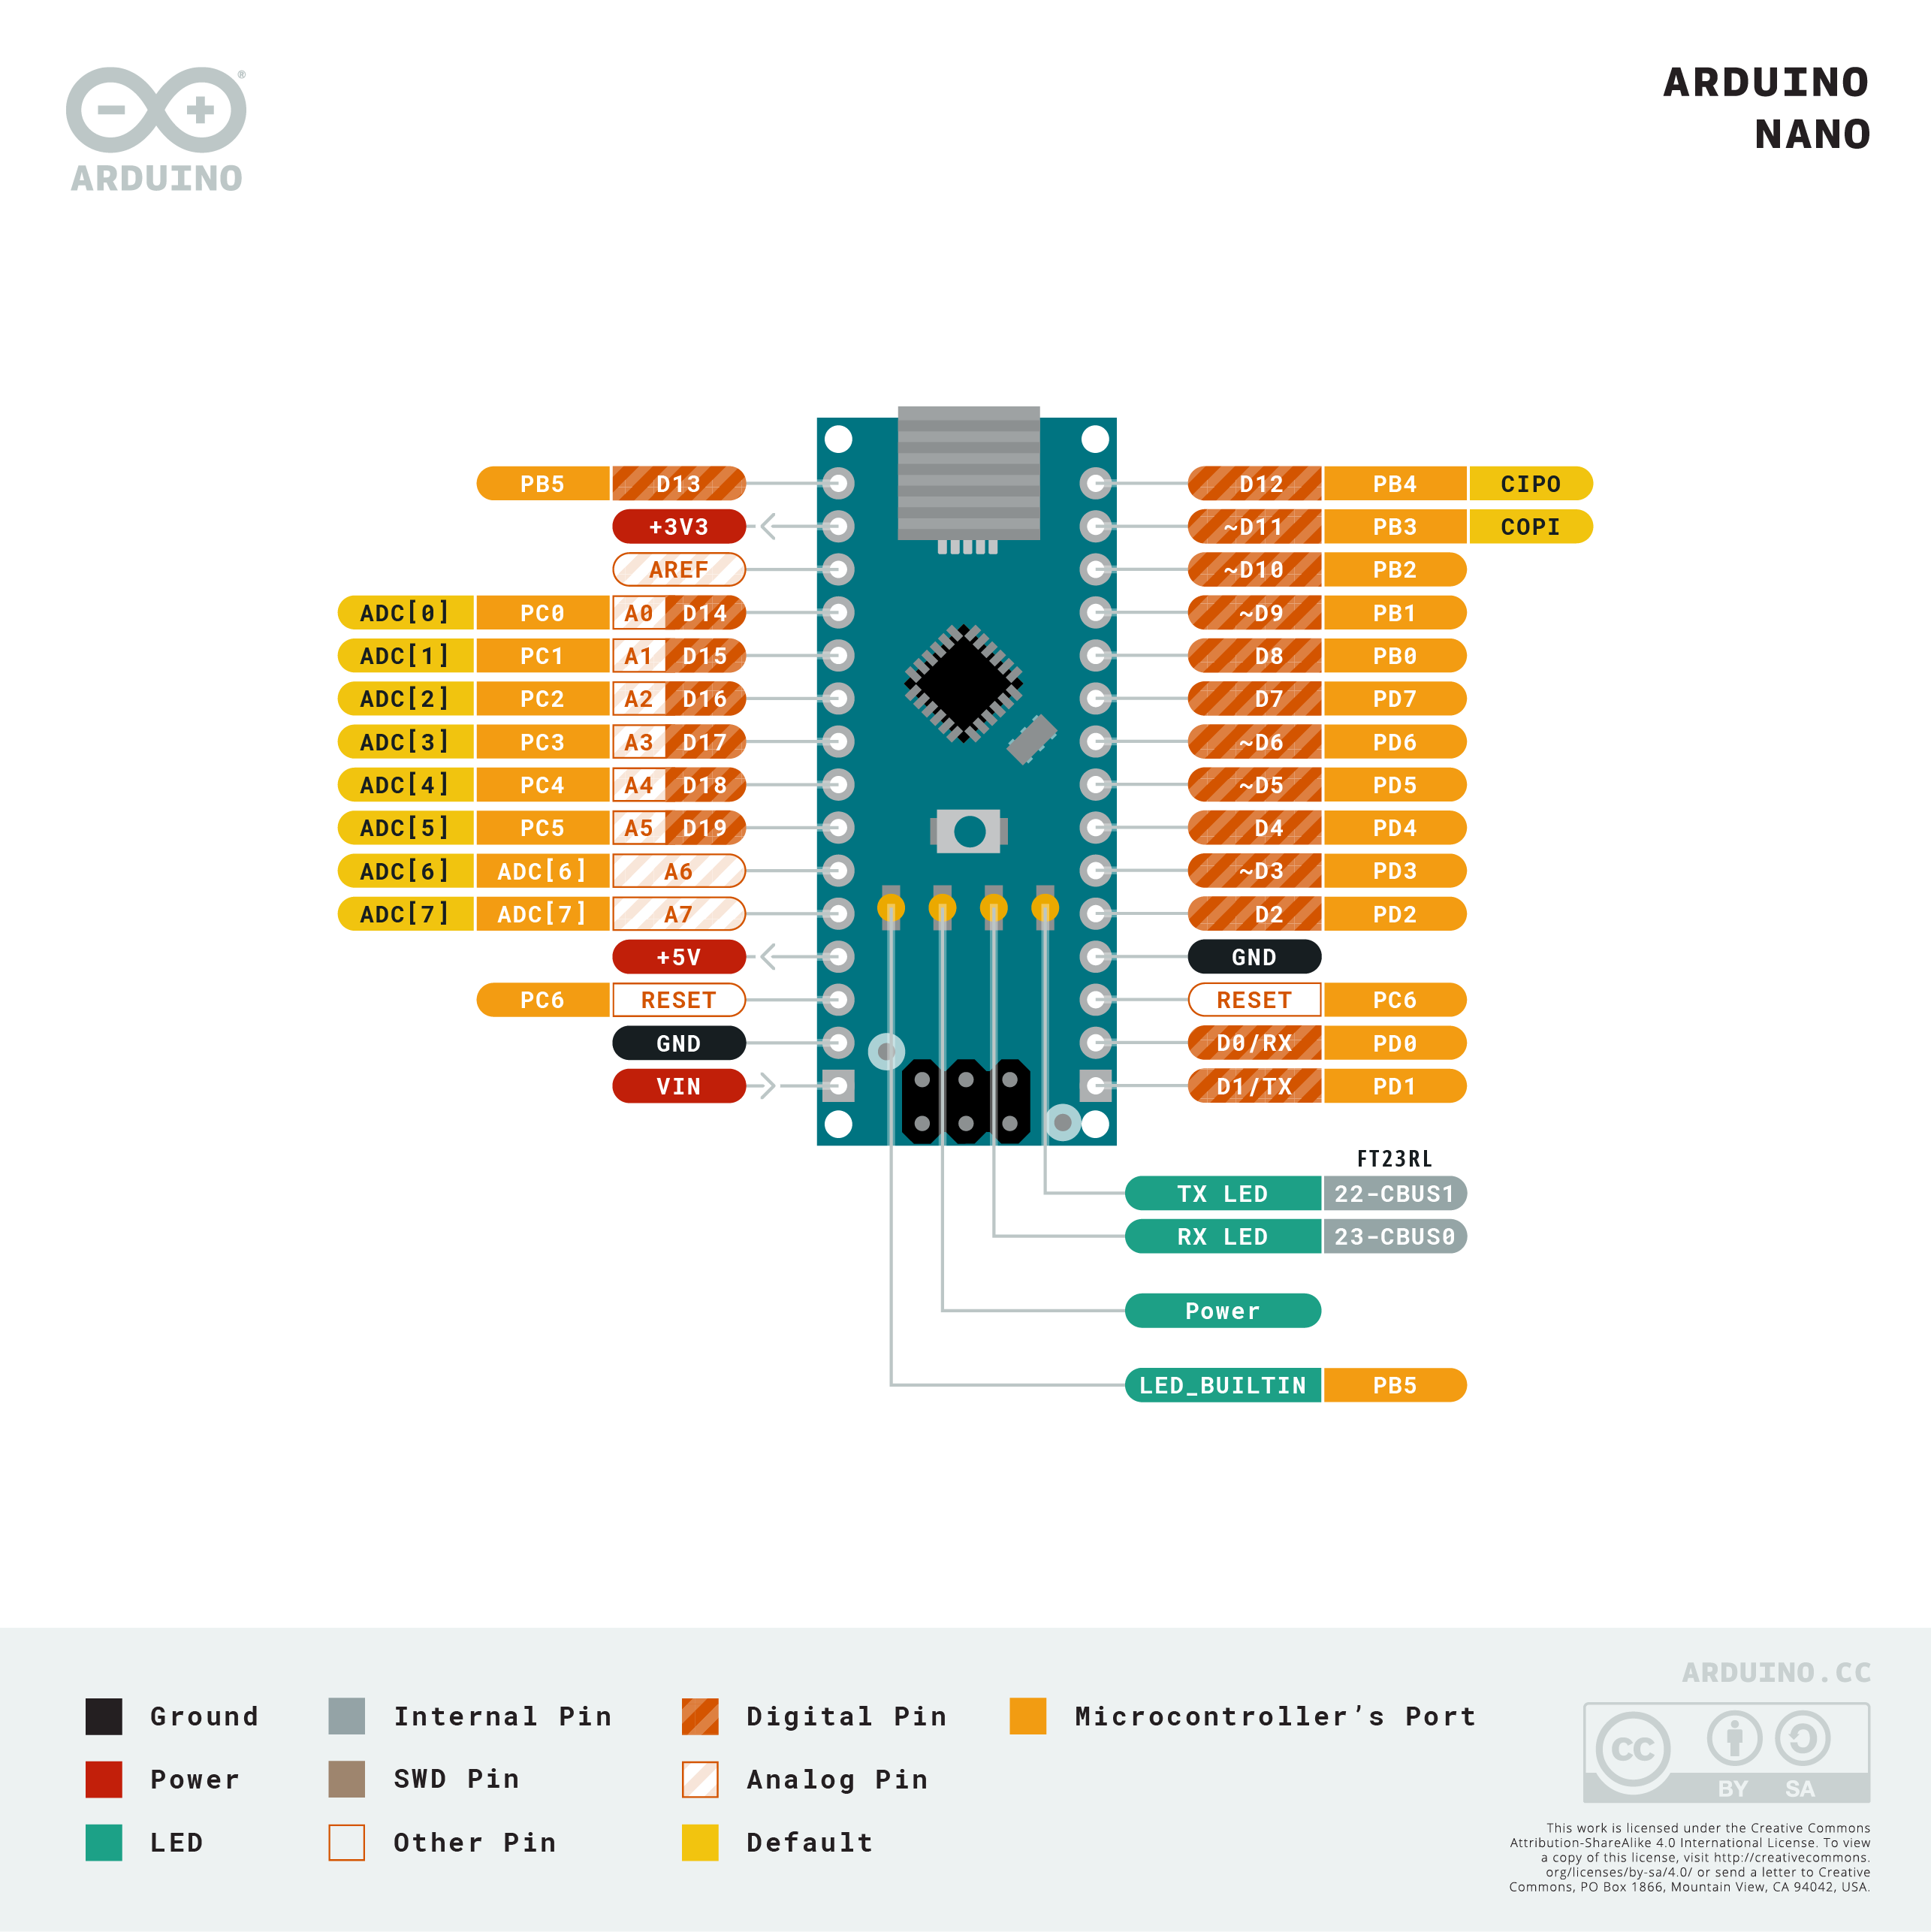
\includegraphics[width=0.7\textwidth]{Imagenes/Bitmap/arduinoNanogpio}
        \caption{Distribución de pines en Arduino Nano}
        \label{fig:arduino_nano_gpio}
    \end{figure}

    Aunque no tiene las capacidades de procesamiento de una Raspberry Pi ni la conectividad integrada del ESP32, el Arduino Nano puede ser una solución válida para CanSat muy simples,
    en los que se priorice el consumo mínimo y no se necesiten funcionalidades avanzadas como WiFi o procesamiento de vídeo, sin embargo, al no tener soporte para cámaras,
    no cumple con los requisitos técnicos necesarios para este proyecto.

\end{itemize}

\begin{table}[h]
    \centering
    \footnotesize
    \resizebox{1.1\textwidth}{!}{
        \begin{tabular}{|l|l|l|l|}
            \hline
            \textbf{Característica} & \textbf{Raspberry Pi Zero 2} & \textbf{ESP32}           & \textbf{Arduino Nano}   \\
            \hline
            Procesador              & ARM Cortex-A53 (4×, 1 GHz)   & Xtensa LX6 (2×, 240 MHz) & ATmega328P (1×, 16 MHz) \\
            \hline
            Memoria                 & 512 MB SDRAM                 & 520 KB SRAM + 4 MB Flash & 2 KB SRAM + 32 KB Flash \\
            \hline
            Wi-Fi                   & Sí                           & Sí                       & No                      \\
            \hline
            Bluetooth               & 4.2 + BLE                    & 4.2 + BLE                & No                      \\
            \hline
            SPI                     & 1                            & 4                        & 1                       \\
            \hline
            I²C                     & 2                            & 2                        & 1                       \\
            \hline
            UART                    & 1                            & 3                        & 1                       \\
            \hline
            Compatibilidad cámara   & CSI (cámara oficial)         & OV2640 (ESP32-CAM)       & No                      \\
            \hline
            Consumo típico          & 0.7--1.5 W                   & 0.2--0.6 W               & 0.05--0.2 W             \\
            \hline
            Precio estimado         & 15--20 €                     & 4--8 €                   & 25--30 €                \\
            \hline
        \end{tabular}}
    \caption{Comparativa de microcontroladores y microcomputadores}
    \label{tab:comparativa-mcus}
\end{table}


\section{Interfaces de comunicación serie}
Una vez analizados sobre los distintos microcontroladores y microprocesadores que existen en el mercado para este tipo de proyectos,
es importante entender los distintos tipos de interfaces de comunicación que utilizan para interactuar con sensores y otros módulos externos y como funcionan.

En esta sección se presentan tres de los más relevantes: SPI, I²C y UART

\begin{itemize}
    \item \textbf{SPI:} La interfaz SPI (Serial Peripheral Interface)~\cite{dhaker_spi} es una interfaz síncrona y full dúplex basada en una arquitectura maestro-esclavo,
    los dos dispositivos, maestro y esclavo pueden transmitir datos simultáneamente sincronizados con una señal de reloj.
    La interfaz SPI utiliza cuatro señales:
    \begin{itemize}
        \item Señal de reloj (CLK)
        \item Selección de chip (CS)
        \item Salida del maestro hacia el esclavo (MOSI)
        \item Salida del esclavo hacia el maestro (MISO)
    \end{itemize}
    \begin{figure}[h]
        \centering
        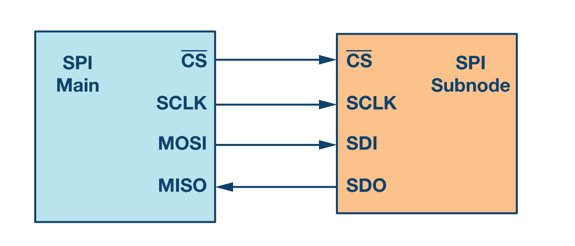
\includegraphics[width=0.8\textwidth]{Imagenes/Bitmap/spi}
        \caption{Configuración SPI con un maestro y un esclavo}
        \label{fig:spi}
    \end{figure}
    El maestro genera la señal de reloj y controla el intercambio de datos.
    El pin CS selecciona el estado activo y los pines MISO y MOSI transportan datos en ambas direcciones.
    Para iniciar la comunicación, el maestro activa el pin CS y empieza a emitir la señal de reloj, al ser una interfaz full dúplex,
    maestro y esclavo pueden enviar y recibir datos simultáneamente.
    Esta interfaz tiene un solo maestro y puede tener uno o múltiples esclavos.
    En configuraciones con múltiples esclavos se pueden conectar de dos modos:
    \begin{itemize}
        \item \textbf{Modo regular:} Cada nodo tiene su propia línea de CS
        \item \textbf{Modo cadena (daisy-chain):} Todos los nodos comparten el mismo reloj y CS y los datos se propagan de un esclavo al siguiente.
        De esta manera se reduce el número de GPIO necesarios en el maestro, aunque aumenta el número de ciclos de reloj requeridos para llegar a cada esclavo.
    \end{itemize}
    La velocidad de transferencia puede variar dependiendo del hardware utilizado, lo habitual es entre 1 y 10Mbps, aunque algunos dispositivos permiten velocidades superiores.

    \item \textbf{I²C:} La interfaz I²C (Inter-Integrated Circuit)~\cite{i2c_specification} es un bus de comunicación síncrono y half dúplex basado en una arquitectura maestro-esclavo, que utiliza solo dos líneas para comunicarse con múltiples dispositivos,
    originalmente fue desarrollada por Philips Semiconductors en 1982.
    Esta interfaz utiliza solo dos señales:
    \begin{itemize}
        \item Línea de datos (SDA)
        \item Línea de reloj (SCL)
    \end{itemize}
    \begin{figure}[h]
        \centering
        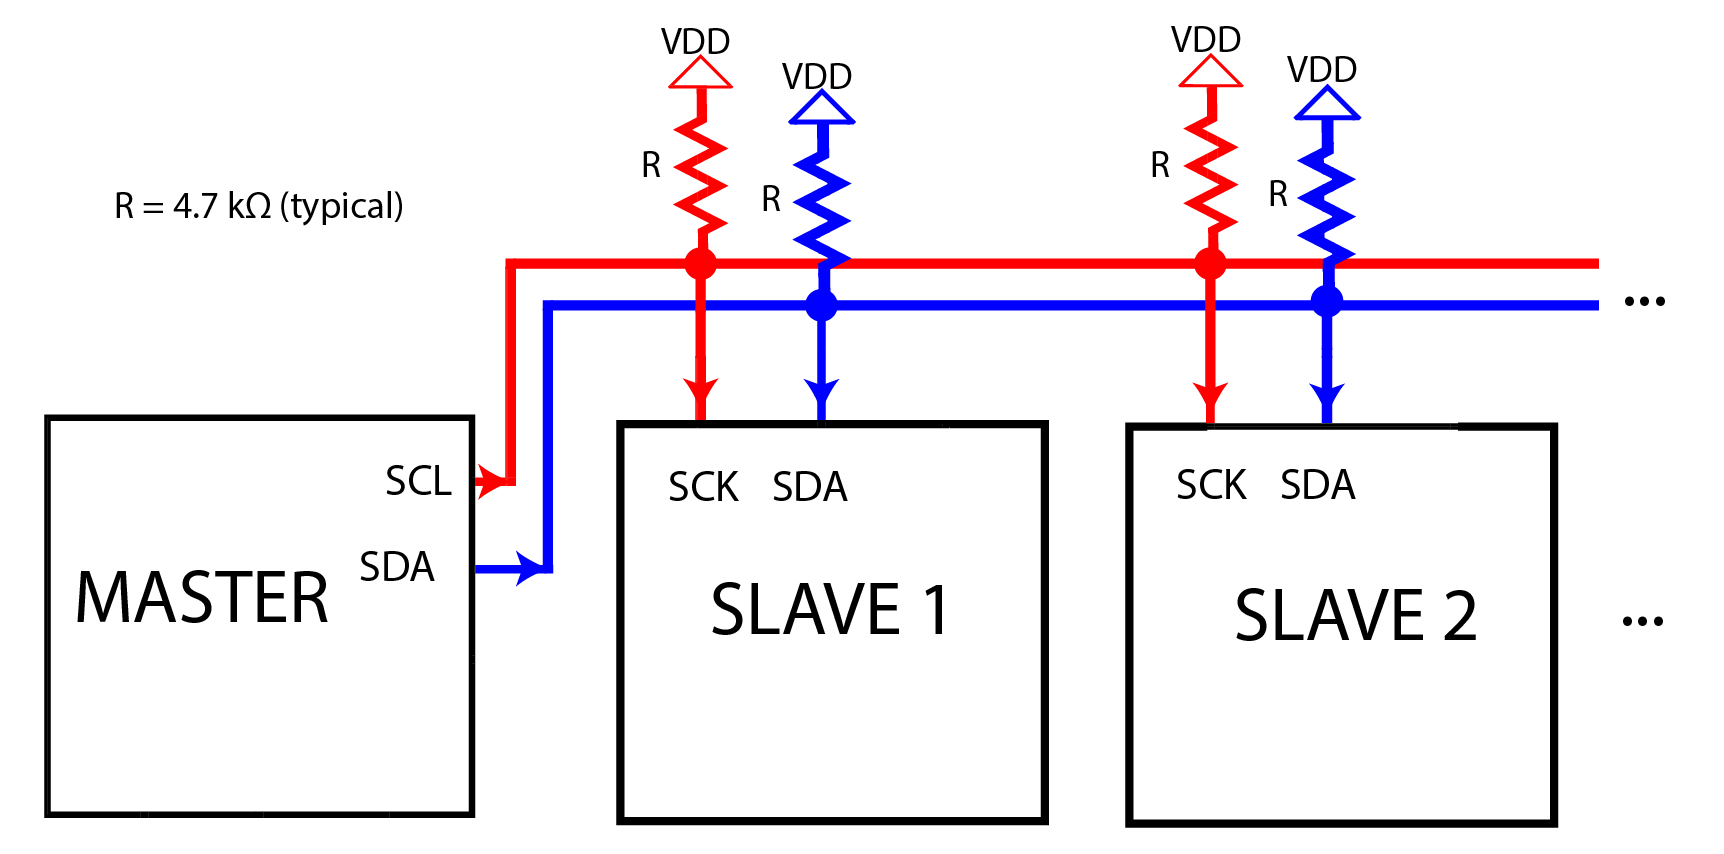
\includegraphics[width=0.8\textwidth]{Imagenes/Bitmap/i2c}
        \caption{Configuración I²C con un maestro y varios esclavos}
        \label{fig:i2c}
    \end{figure}
    Ambas líneas son bidireccionales aunque al ser half dúplex la comunicación se realiza en un sentido a la vez.
    Un dispositivo actúa como maestro, iniciando la comunicación y generando la señal de reloj, mientras que uno o más esclavos responden.
    Cada dispositivo conectado al bus tiene una dirección única.

    La comunicación se inicia cuando el maestro envía una condición de inicio, la dirección de uno de los dispositivos conectados al bus y un bit indicando si va a leer o escribir.
    Después de transmitir cada byte, el receptor envía una señal de reconocimiento (ACK). La transmisión termina cuando se envía una condición de parada.

    El bus I²C permite velocidades de transferencia de hasta 100 kbit/s en modo estándar (Standard-mode), 400 kbit/s en modo rápido (Fast-mode), 1 Mbit/s en modo fast-mode plus (Fm+), y hasta 3.4 Mbit/s en modo high-speed (Hs-mode), dependiendo de las capacidades del hardware.

    \item \textbf{UART:} La interfaz UART (Universal Asynchronous Receiver-Transmitter)~\cite{infineon_uart} es una interfaz de comunicación asíncrona basada en una arquitectura punto a punto,
    que permite la transmisión de datos en serie entre dos dispositivos.
    A diferencia de las interfaces anteriores, que eran síncronas, UART es asíncrona, por lo que no utiliza una señal de reloj compartida,
    sino que cada dispositivo funciona con una velocidad de transmisión acordada previamente y común para los dos (baud rate).
    UART emplea dos líneas de comunicación:
    \begin{itemize}
        \item Transmisión de datos (TX)
        \item Recepción de datos (RX)
    \end{itemize}
    \begin{figure}[h]
        \centering
        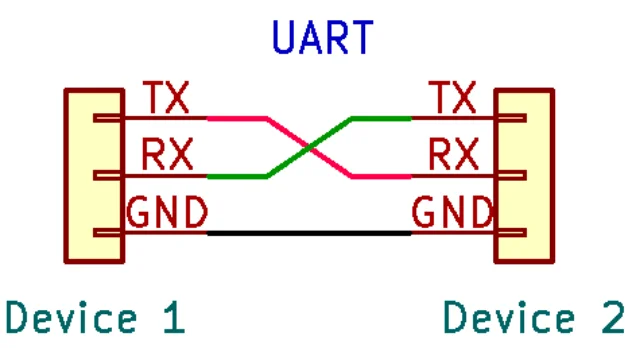
\includegraphics[width=0.8\textwidth]{Imagenes/Bitmap/uart}
        \caption{Ejemplo de conexión UART}
        \label{fig:uart}
    \end{figure}
    La línea TX de un dispositivo debe ir conectada a la línea RX del otro dispositivo, y la línea RX a TX.

    La comunicación es full dúplex, permitiendo la transmisión y recepción de datos de forma simultánea.
    Cada byte se transmite en una trama que incluye un bit de inicio (start bit), los bits de datos (normalmente 8), un bit opcional de paridad, y uno o más bits de parada (stop bits).

    Las velocidades de transmisión habituales van desde 9600 hasta 115200 baudios, aunque se pueden alcanzar velocidades de hasta 1 o 2 Mbps, dependiendo del hardware.

\end{itemize}

\begin{table}[h]
    \centering
    \footnotesize
    \renewcommand{\arraystretch}{1.1}
    \begin{tabular}{|l|c|c|c|}
        \hline
        \textbf{Característica} & \textbf{SPI}               & \textbf{I²C}               & \textbf{UART}       \\
        \hline
        Tipo de comunicación    & Síncrona                   & Síncrona                   & Asíncrona           \\
        \hline
        Arquitectura            & Maestro-esclavo            & Maestro-esclavo            & Punto a punto       \\
        \hline
        Número de líneas        & 4 (CLK, CS, MOSI, MISO)    & 2 (SDA, SCL)               & 2 (TX, RX)          \\
        \hline
        Full/Half dúplex        & Full dúplex                & Half dúplex                & Full dúplex         \\
        \hline
        Número de dispositivos  & 1 maestro, varios esclavos & 1 maestro, varios esclavos & Solo dos            \\
        \hline
        Velocidad típica        & 1–10 Mbps                  & 100 kbit/s – 3.4 Mbit/s    & 9.6 kbit/s – 3 Mbps \\
        \hline
        Control de dirección    & Señal CS por esclavo       & Dirección en el protocolo  & No necesario        \\
        \hline
    \end{tabular}
    \caption{Comparativa entre las interfaces SPI, I²C y UART}
    \label{tab:comparativa_interfaces}
\end{table}


\section{Tecnologías de comunicación por radiofrecuencia en sistemas embebidos}
Dentro de los sistemas embebidos y en particular en sistemas tipo CanSat es muy importante la comunicación inalámbrica entre el satélite y la estación de tierra.
De entre las diversas opciones de comunicación inalámbrica, en este apartado vamos a estudiar las distintas opciones que hay en el mercado de comunicación por radiofrecuencia.
Este tipo de comunicación nos ofrece un largo alcance manteniendo el bajo consumo, un aspecto muy relevante en un CanSat.

Las tres opciones de comunicación por radiofrecuencia que vamos a estudiar son:

\begin{itemize}
    \item \textbf{LoRa:} La tecnología (Long Range)~\cite{augustin_lora} permite una comunicación inalámbrica de largo alcance con un bajo consumo energético,
    forma parte de las LPWAN (Low-Power Wide-Area Network) redes orientadas a aplicaciones de internet de las Cosas (IoT).

    Técnicamente, Lora funciona utilizando una tecnología de modulación de espectro ensanchado basada en chirp spread spectrum (CSS).
    Cada símbolo(conjunto de bits transmitidos como una única unidad) se transmite mediante un único chirp, es decir,
    una señal cuya frecuencia varía linealmente (aumentando o disminuyendo) a lo largo del tiempo.
    El número de bits por símbolo se determina por el Spreading Factor (SF), de modo que un SF de 7 bits codifica 7 bits por símbolo,
    un SF de 10 codifica 10 bits, y así sucesivamente.

    Además, LoRa incorpora un esquema de corrección de errores hacia adelante (Forward Error Correction, FEC), que mejora la fiabilidad de la comunicación en entornos con ruido o interferencias.
    Este sistema añade bits redundantes a los datos transmitidos, permitiendo al receptor detectar y corregir errores sin necesidad de retransmisión.
    La cantidad de redundancia depende de la tasa de codificación (Coding Rate, CR), que puede configurarse entre 4/5 y 4/8.
    Esta tasa indica cuántos bits útiles se transmiten por cada bloque de bits totales.
    Por ejemplo, una tasa de 4/5 significa que por cada 5 bits enviados, 4 contienen información útil y 1 es redundante para corrección de errores.
    De forma similar, una tasa de 4/8 implica que solo 4 de cada 8 bits son datos útiles y los 4 restantes son bits de corrección.
    Cuanto menor es la tasa, mayor es la redundancia y, por tanto, mayor la robustez frente a errores, aunque la velocidad efectiva de transmisión es menor.

    Opera en bandas de frecuencia no licenciadas, como 433 MHz, 868 MHz (Europa) o 915 MHz (América),
    esto permite su uso sin coste dentro de este espectro.

    El alcance varía dependiendo del entorno, desde cientos de metros en entornos urbanos con muchas interferencias hasta más de 15 kilómetros en entornos abiertos y despejados.

    \item  \textbf{XBee:} Los módulos XBee ~\cite{digi_xbee_15_4} han sido desarrollados por Digi International y permiten establecer comunicaciones inalámbricas de corto a medio alcance
    con bajo consumo energético.
    Utilizan el estándar IEEE 802.15.4 para las capas física y MAC, lo que les proporciona interoperabilidad con otros dispositivos compatibles con este estándar.

    Estos módulos operan en la banda ISM de 2.4GHz utilizando modulación DSSS (Direct Sequence Spread Spectrum) con O-QPSK (Offset Quadrature Phase Shift Keying), alcanzando una tasa de transferencia aérea de 250kbps.

    La técnica \textit{DSSS} consiste en dispersar cada bit de datos sobre una secuencia de mayor ancho de banda mediante una secuencia pseudoaleatoria (chipping code), lo que proporciona robustez frente a interferencias y permite que múltiples transmisiones compartan el mismo canal sin colisiones significativas.

    Por su parte, \textit{O-QPSK} es una variante de la modulación por desplazamiento de fase en cuadratura (QPSK), que introduce un desfase temporal entre las componentes en fase y en cuadratura para reducir los cambios bruscos en la señal transmitida,
    mejorando así la eficiencia espectral y reduciendo la probabilidad de errores durante la demodulación.

    Digi ha desarrollado interfaces de configuración y modos de operación propios, como el modo API, que encapsula datos y comandos en tramas estructuradas para control avanzado,
    además del modo transparente, que permite una comunicación directa punto a punto.

    XBee permite topologías de red como punto a punto o estrella.
    Cada módulo tiene una dirección MAC única de 64 bits y puede asignarse una dirección corta de 16 bits para identificación dentro de la red.
    La comunicación con el microcontrolador suele realizarse mediante UART, con velocidades configurables de hasta 1Mbps.

    En condiciones óptimas, el alcance puede variar entre 30 y 100 metros en interiores, y superar los 300 metros en exteriores.
    \item \textbf{APC220:} El módulo APC220~\cite{apc220_datasheet} es un transceptor de radiofrecuencia desarrollado por Appcon Technologies que permite establecer comunicaciones inalámbricas punto a punto en sistemas embebidos de bajo consumo.
    Este módulo opera en la banda ISM de 433 MHz lo que hace que no necesite licencia para funcionar.

    El APC220 emplea modulación GFSK (Gaussian Frequency Shift Keying), una variante de FSK (Frequency Shift Keying) en la que las transiciones de frecuencia entre los niveles binarios (0 y 1) se suavizan usando un filtro gaussiano aplicado previamente a la señal digital.
    Esta técnica reduce la anchura de banda de la señal transmitida y minimiza las emisiones fuera de banda, lo que se traduce en menor interferencia con otros sistemas y una mayor eficiencia espectral.
    Además, GFSK mejora la robustez frente al ruido, mejorando su eficiencia en entornos con interferencias.

    La tasa de transmisión es configurable entre 1200 bps y 19200 bps, utilizando UART como interfaz con el microcontrolador.

    El módulo integra un amplificador de potencia y un receptor de alta sensibilidad, permitiendo un alcance de hasta 1000 metros en condiciones óptimas con línea de visión clara.
    Además, incluye un circuito interno de corrección de errores y control automático de ganancia (AGC), que mejoran la fiabilidad de la comunicación.

    Su configuración puede ajustarse mediante comandos AT o mediante una herramienta software proporcionada por el fabricante, conectando el módulo a través de un convertidor USB-UART
\end{itemize}
\begin{table}[h]
    \centering
    \footnotesize
    \begin{tabular}{|l|c|c|c|}
        \hline
        \textbf{Característica} & \textbf{LoRa}                   & \textbf{XBee (802.15.4)} & \textbf{APC220}    \\
        \hline
        Frecuencia de operación & 433/868/915 MHz                 & 2.4 GHz                  & 433 MHz            \\
        \hline
        Modulación              & CSS (Chirp Spread Spectrum)     & DSSS + O-QPSK            & GFSK               \\
        \hline
        Velocidad de datos      & 0.3–27 kbps                     & 250 kbps                 & 1.2–19.2 kbps      \\
        \hline
        Alcance típico          & Hasta 15 km (entornos abiertos) & 30–300 m                 & Hasta 1 km         \\
        \hline
        Corrección de errores   & FEC configurable (CR 4/5–4/8)   & No especificado          & FEC + AGC internos \\
        \hline
        Interfaz con MCU        & UART                            & UART                     & UART               \\
        \hline
        Topología de red        & Punto a punto                   & Punto a punto / estrella & Punto a punto      \\
        \hline
    \end{tabular}
    \caption{Comparativa de tecnologías de comunicación por radiofrecuencia}
    \label{tab:comparativa_rf}
\end{table}


\section{Sensores empleados para telemetría: presión barométrica, IMU y GNSS}
A continuación se describen de los distintos tipos sensores empleados para cumplir con los requisitos del CanSat.
Estos sensores son los encargados de tomar mediciones precisas sobre distintas variables del entorno.
Para cumplir con estos requisitos se requiere la integración de tres tipos distintos de sensores:
\begin{itemize}
    \item \textbf{Presión barométrica:} Los sensores de presión barométrica se utilizan para medir la presión atmosférica y de esta forma estimar la altura sobre el nivel del mar mediante modelos estándar como el ISA (International Standard Atmosphere)~\cite{skybrary_isa}.

    La presión atmosférica es la fuerza que ejerce el peso de una columna de aire sobre un área determinada,
    por ello, al medir la presión sobre un punto de la tierra con mayor altitud la presión será menor por ser menor la cantidad de aire sobre ese punto.

    Distintos factores meteorológicos pueden hacer variar la presión atmosférica, principalmente con los cambios de temperatura,
    al variar la temperatura, varía la densidad del aire y, por lo tanto, varía su peso, afectando a la presión.

    Otros factores como la humedad relativa o el viento también influyen aunque de menor manera y pueden ser obviados.

    En el mercado se pueden encontrar distintos modelos de estos sensores, que varían entre ellos en función de su precisión, interfaz de conexión con el microcontrolador, consumo energético y precio.
    \begin{table}[h]
        \centering
        \footnotesize
        \begin{tabular}{|l|c|c|c|c|c|}
            \hline
            \textbf{Sensor} & \textbf{Rango de presión} & \textbf{Precisión} & \textbf{Interfaz}          & \textbf{Consumo típico} & \textbf{Precio (€)} \\
            \hline
            BMP388          & 300–1250 hPa              & ±8 Pa (±0.66 m)    & I\textsuperscript{2}C, SPI & 3.4 µA                  & \textasciitilde3.50 \\
            \hline
            BME280          & 300–1100 hPa              & ±12 Pa (±1 m)      & I\textsuperscript{2}C, SPI & 2.7 µA                  & \textasciitilde4.00 \\
            \hline
            MPL3115A2       & 50–1100 hPa               & ±0.04 hPa (±0.3 m) & I\textsuperscript{2}C      & 40 µA                   & \textasciitilde6.00 \\
            \hline
        \end{tabular}
        \caption{Comparativa de sensores de presión barométrica}
        \label{tab:barometric_sensors}
    \end{table}


    \item \textbf{IMU:} Una unidad de medición inercial o IMU, es un dispositivo que mide la velocidad, orientación y fuerzas gravitacionales de un aparato,
    para hacerlo generalmente utiliza una combinación de sensores, acelerómetros y giroscopios.

    Para su funcionamiento utiliza tres acelerómetros colocados de tal forma que sus ejes de medición queden de manera ortogonal entre sí,
    estos acelerómetros se utilizan para medir las fuerzas de aceleración (fuerzas G) que actúan en cada eje.

    También cuenta con tres giróscopios colocados en un patrón ortogonal similar, estos giróscopios miden la velocidad angular alrededor de cada eje, permitiendo conocer los cambios en la orientación del objeto respecto a un sistema de referencia.

    Algunos modelos también pueden contar con un magnetómetro, que mide el campo magnético terrestre y permite estimar el rumbo respecto al norte magnético.

    La combinación de estos sensores nos permite conocer la orientación en el espacio de un objeto en términos de los tres ángulos de Euler: pitch, yaw, y roll muy utilizados en aplicaciones aeronáuticas y espaciales.
    \begin{figure}[h]
        \centering
        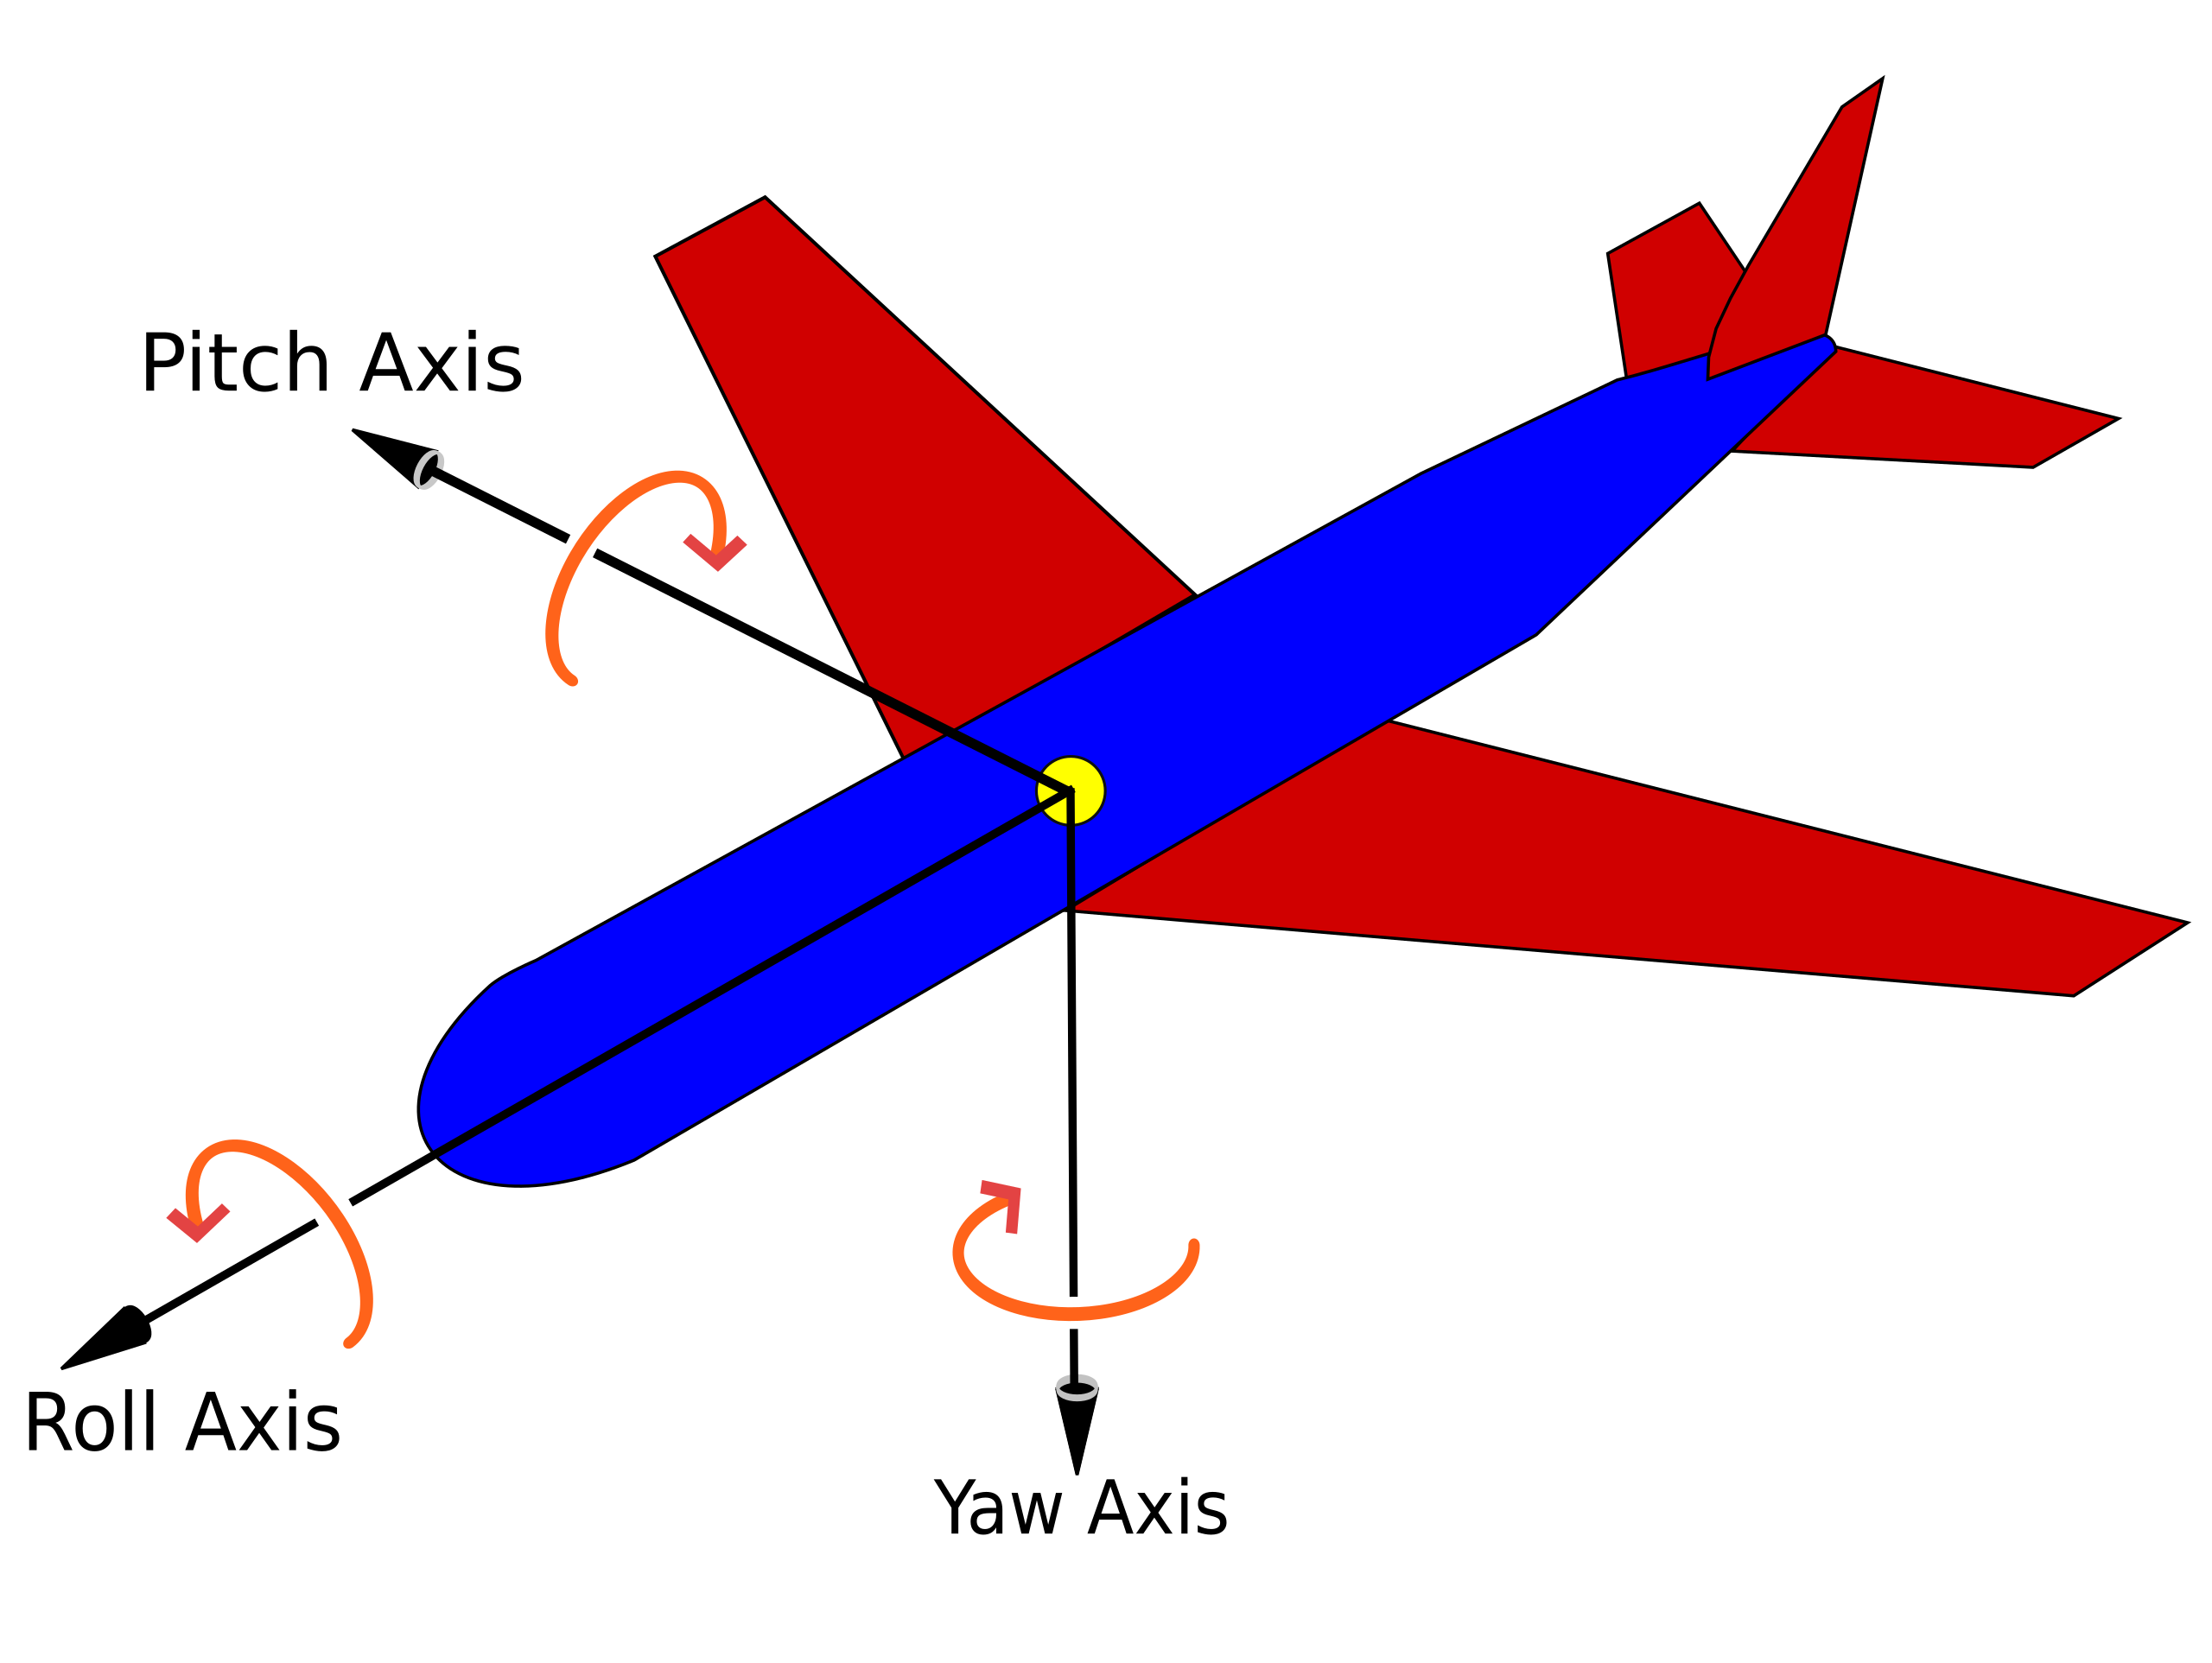
\includegraphics[width=0.8\textwidth]{Imagenes/Bitmap/pitch_yaw_roll}
        \caption{Sistema de referencia basado en los ángulos de pitch, yaw y roll}
        \label{fig:pitch_yaw_roll}
    \end{figure}

    En algunos modelos de sensores disponibles en el mercado, esta combinación de sensores viene acompañada de un procesador interno que realiza fusión sensorial,
    permitiendo obtener directamente la orientación del dispositivo sin necesidad de cálculos externos.

    \begin{table}[h]
        \centering
        \resizebox{1.15\textwidth}{!}{
            \begin{tabular}{|l|c|c|c|c|c|}
                \hline
                \textbf{Sensor} & \textbf{Componentes}                     & \textbf{Salida de orientación}        & \textbf{Interfaz} & \textbf{Consumo típico} & \textbf{Precio (€)} \\
                \hline
                MPU6050         & Acelerómetro + Giroscopio                & No (requiere procesamiento externo)   & I\textsuperscript{2}C & 3.9 mA & \textasciitilde1.50 \\
                \hline
                BNO055          & Acelerómetro + Giroscopio + Magnetómetro & Sí (procesamiento interno con fusión) & I\textsuperscript{2}C / UART & 12 mA & \textasciitilde9.00 \\
                \hline
                BNO085          & Acelerómetro + Giroscopio + Magnetómetro & Sí (mejor precisión que BNO055)       & I\textsuperscript{2}C / UART / SPI & 3.5 mA & \textasciitilde14.00 \\
                \hline
                LSM9DS1         & Acelerómetro + Giroscopio + Magnetómetro & No (requiere fusión externa)          & I\textsuperscript{2}C / SPI & 1.0 mA & \textasciitilde5.00 \\
                \hline
            \end{tabular}
        }
        \caption{Comparativa de sensores IMU}
        \label{tab:imu_comparison}
    \end{table}

    \item \textbf{GNSS:} Global Navigation Satellite System~\cite{inertiallabs_gnss} es un sistema de navegación por satélite que engloba las siguientes constelaciones de satélites:
    GPS (Estados Unidos)~\cite{gps_system}, Galileo (Europa)~\cite{galileo_system}, GLONASS (Rusia)~\cite{glonass_system}y BeiDou (China)~\cite{beidou_system}.
    \begin{table}[h]
        \centering
        \footnotesize
        \begin{tabular}{|l|c|c|c|c|}
            \hline
            \textbf{Sistema} & \textbf{País / Región} & \textbf{Satélites operativos} & \textbf{Precisión típica (civil)} & \textbf{Frecuencias principales} \\
            \hline
            GPS              & Estados Unidos         & 31                            & 5–10 metros                       & L1, L2, L5                       \\
            \hline
            Galileo          & Unión Europea          & 28                            & <1 metro (con E5 AltBOC)          & E1, E5a, E5b, E6                 \\
            \hline
            GLONASS          & Rusia                  & 24                            & 5–10 metros                       & L1, L2                           \\
            \hline
            BeiDou           & China                  & 45                            & 2.5–5 metros                      & B1, B2, B3                       \\
            \hline
        \end{tabular}
        \caption{Comparativa de las principales constelaciones GNSS}
        \label{tab:gnss_constellations}
    \end{table}


    Estos sistemas se utilizan para determinar la posición geográfica y la velocidad de un objeto en cualquier parte del planeta utilizando estas constelaciones de satélites.
    Para determinar la posición y velocidad se necesita un receptor GNSS que recibe las señales emitidas por los satélites que contienen información sobre su posición y la fecha exacta en la que fueron enviadas.
    Cuando el receptor recibe señales de al menos tres satélites, puede calcular su posición usando una técnica geometrica llamada trilateración~\cite{trilateracion}.

    \begin{figure}[h]
        \centering
        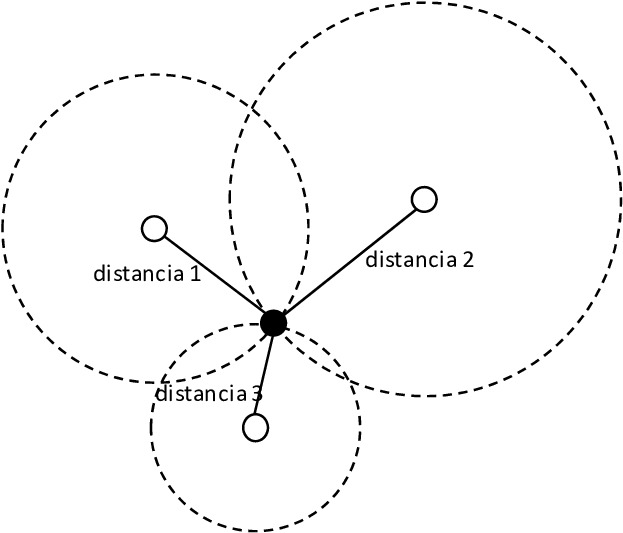
\includegraphics[width=0.7\textwidth]{Imagenes/Bitmap/trilateracion}
        \caption{Ejemplo de cálculo de la posición usando la técnica trilateración}
        \label{fig:trilateracion}
    \end{figure}

    Esta técnica permite conocer la posición de un objeto conociendo su distancia a tres puntos de referencia,
    en este caso, estos tres puntos son las posiciones de los satélites.

    Actualmente, en el mercado existe una gran variedad de receptores GNSS diseñados para aplicaciones embebidas, que varían en su precisión, consumo, constelaciones soportadas y coste.
    A continuación se muestra una comparativa entre algunos de los receptores GNSS más comunes.
    \begin{table}[h]
        \centering
        \footnotesize
        \resizebox{1.15\textwidth}{!}{
            \begin{tabular}{|l|c|c|c|c|c|}
                \hline
                \textbf{Módulo} & \textbf{Constelaciones soportadas}      & \textbf{Precisión típica} & \textbf{Frecuencia de actualización} & \textbf{Consumo} & \textbf{Precio aprox.} \\
                \hline
                BN-880          & GPS, GLONASS, Galileo, BeiDou           & ~2m CEP                   & 1--10Hz                              & ~50mA a 5V       & ~15--25€               \\
                \hline
                NEO-M8N         & GPS, GLONASS, Galileo, BeiDou           & ~2m CEP                   & hasta 18Hz                           & <150mA a 5V      & ~35--40€               \\
                \hline
                NEO-F9P         & GPS, GLONASS, Galileo, BeiDou (con RTK) & cm-level con RTK          & hasta 20Hz                           & ~100mA a 3.3V & ~110--130€ \\
                \hline
            \end{tabular}
        }
        \caption{Comparativa de receptores GNSS comunes en sistemas embebidos}
        \label{tab:gnss_modules}
    \end{table}


\end{itemize}


\section{Captura y transmisión de vídeo en tiempo real}
Como parte de los requisitos para este proyecto CanSat se encuentra la transmisión de vídeo, pudiendo ser visualizada en tiempo real desde una plataforma web.

Para llevar a cabo esto, estudiaremos los fundamentos técnicos de la captura digital de video, las distintas maneras de códificarla, los distintos formatos de contenedor y los principales protocolos de transmisión en tiempo real.

\subsection{Captura digital de vídeo}
La captura digital de vídeo es el proceso mediante el cual una cámara convierte la luz del entorno en información digital que puede ser procesada y almacenada.
Este proceso se realiza mediante un sensor de imágen, que transforma la luz en señales eléctricas.

Existen principalmente dos tipos de sensores usados en este tipo de sistemas de este tipo:
\begin{itemize}
    \item \textbf{CMOS:} Los sensores CMOS (Complementary Metal-Oxide-Semiconductor)~\citep{cmos}, fueron desarrollados en 1993 como una alternativa más eficiente y económica a los sensores CCD

    Funcionan mediante una matriz de fotodiodos que convierten la luz incidente en carga eléctrica.
    Cada píxel del sensor incorpora circuitos activos que amplifican y digitalizan la señal generada, lo que permite leer simultáneamente múltiples píxeles en paralelo.

    Los sensores CMOS actuales cuentan con conversores analógico-digitales (ADC) y procesado de imagen incluídos en el propio chip, lo que disminuye el ruido y mejora el rendimiento en condiciones de baja iluminación.
    \item \textbf{CCD:}Los sensores CCD (Charge-Coupled Device)~\citep{blanc2001ccd} fueron desarrollados en 1969 por Willard Boyle y George E. Smith.

    A diferencia de los sensores CMOS, en los CCD la luz incide sobre una matriz de fotodiodos que convierte los fotones en carga eléctrica, pero esta carga no se convierte inmediatamente en una señal digital.
    En su lugar, se transfiere secuencialmente a lo largo del chip mediante registros de desplazamiento hasta llegar a una única etapa de conversión analógico-digital

    Esto lo convierte en un proceso más lento y con mayor consumo energético.
\end{itemize}
Dentro de la cáptura de video encontramos algunos parámetros importantes:
\begin{itemize}
    \item \textbf{Resolución:} número de píxeles de cada fotograma (por ejemplo, 640x480 o 1920x1080) y determina el nivel de detalle de la imagen.
    \item \textbf{Tasa de fotogramas (fps):} indica el número de fotogramas por segundo, y afecta a la fluidez del vídeo.
\end{itemize}

Una vez obtenidos los datos del sensor, se sigue un proceso de codificación del vídeo, en este proceso se comprime los datos brutos para reducir su tamaño pero manteniendo una buena calidad de imagen.

Estos son los codecs (formatos de compresión) más comunes:
\begin{itemize}
    \item \textbf{H.264 (AVC):} El códec H.264 (también conocido como AVC, Advanced Video Coding)\cite{H.264} es un estándar de compresión de vídeo con pérdida,

    Divide cada fotograma en macrobloques, que se analizan para aprovechar redundancias temporales (entre fotogramas) y espaciales (dentro de un mismo fotograma).

    Usando esta técnica, puede alcanzar una alta relación de compresion sin comprometer demasiado la calidad de imagen.

    \item \textbf{H.265 (HEVC):} El códec H.265 o HEVC (High Efficiency Video Coding)~\cite{hevc_h265} es el sucesor directo de H.264, está diseñado para ofrecer el mismo nivel de calidad que su antecesor,
    utilizando aproximadamente la mitad del bitrate.

    Para ello utiliza bloques de compresión más grandes y mayor profundidad de predicción, además soporta resoluciones de hasta 8K, para lograr esto necesita mayor capacidad de procesamiento, tanto al codificar como al decodificar.

    \item \textbf{MJPEG (Motion JPEG):}~\cite{mjpeg_codec}, Codifica cada fotograma de vídeo como una imagen JPEG independiente.

    A diferencia de los códecs anteriores no se beneficia de las redundancias entre fotogramas, sin embargo, es más simple y rápido, por lo que necesita menos capacidad de procesamiento y provoca una menor latencia.

\end{itemize}
\begin{table}[h]
    \centering
    \footnotesize
    \begin{tabular}{|l|c|c|c|}
        \hline
        \textbf{Códec} & \textbf{Compresión} & \textbf{Requiere procesamiento elevado} & \textbf{Latencia} \\
        \hline
        H.264 (AVC)    & Alta                & Media                                   & Baja              \\
        \hline
        H.265 (HEVC)   & Muy alta            & Alta                                    & Media             \\
        \hline
        MJPEG          & Baja                & Baja                                    & Muy baja          \\
        \hline
    \end{tabular}
    \caption{Comparativa entre códecs de vídeo comunes}
    \label{tab:video_codecs}
\end{table}

Los codecs definen como se comprime la imagen, pero no como se almacenan esos datos, para ello se utilizan formatos contenedores.

Un formato contenedor es un formato de archivo que encapsula uno o m/as flujos de datos codificados, normalmente video y audio, junto con la información necesaria para sincronizarlos y reproducirlos correctamente.

Algunos de los formatos contenedores más comunes incluyen:

\begin{itemize}
    \item \textbf{AVI (Audio Video Interleave):} Formato contenedor desarrollado por Microsoft en 1992.
    Presenta limitaciones para la transmisión en tiempo leal y no soporta bien múltiples pistas de audio o subtítulos.

    \item \textbf{MP4 (MPEG-4 Part 14):} Uno de los formatos más utilizados actualmente.
    Soporta vídeo (principalmente H.264/H.265), audio, subtítulos y metadatos.
    Es ideal para transmisión y almacenamiento, y es compatible con casi todos los navegadores y plataformas.

    \item \textbf{MKV (Matroska):} Formato contenedor libre y flexible, capaz de contener múltiples flujos de vídeo, audio y subtítulos en un solo archivo.
    Es muy utilizado para contenidos de alta calidad, aunque su compatibilidad es más limitada.

    \item \textbf{FLV (Flash Video):} Fue diseñado originalmente para la transmisión de vídeo a través de Adobe Flash.
    Soporta códecs como H.264 y es ampliamente utilizado en plataformas streaming.
    Se utiliza sobre todo en sistemas que emplean el protocolo RTMP debido a su baja latencia.
\end{itemize}

\begin{table}[h]
    \centering
    \footnotesize
    \begin{tabular}{|l|c|c|c|c|}
        \hline
        \textbf{Formato} & \textbf{Códecs comunes}  & \textbf{Soporte multitrack} & \textbf{Uso típico}                  \\
        \hline
        AVI              & H.264, MJPEG, DivX       & Limitado                    & Almacenamiento local                 \\
        \hline
        MP4              & H.264, H.265 (HEVC), AAC & Sí                          & Transmisión y almacenamiento         \\
        \hline
        MKV              & H.264, H.265, VP9, Opus  & Sí                          & Contenido multimedia de alta calidad \\
        \hline
        FLV              & H.264, MP3, AAC          & Limitado                    & Transmisión en tiempo real (RTMP)    \\
        \hline
    \end{tabular}
    \caption{Comparativa de formatos contenedores de vídeo}
    \label{tab:video_containers}
\end{table}

\subsection{Protocolos de transmisión de vídeo en tiempo real}
Los protocolos en tiempo real permiten enviar vídeo y audio a través de redes IP de manera continua,
permitiendo la visualización del contenido con la menor latencia posible.

A continuación se describen los principales protocolos utilizados en este contexto:

\begin{itemize}
    \item \textbf{RTMP (Real-Time Messaging Protocol):} El protocolo RTMP~\citep{rtmp_adobe} funciona sobre TCP, normalmente usando el puerto 1935 y establece una conexión persistente entre cliente y servidor.

    Utiliza multiplexación a nivel de protocolo para dividir el flujo continuo en pequeños (chunks) de datos que intercalan vídeo, audio y comandos de control,
    lo que permite mantener una única conexión TCP
    Este diseño permite mantener una latencia baja, normalmente entre 3 y 5 segundos.

    La conexión comienza con un intercambio de mensajes (handshake) entre cliente y servidor, seguido por comandos codificados en formato AMF para controlar la transmisión.

    A diferencia de protocolos como HLS o DASH que segmentan el vídeo en archivos, RTMP divide el flujo en chunks internos multiplexados con vídeo, audio y control.

    \item \textbf{HLS (HTTP Live Streaming):} El protocolo HLS~\citep{hls_ietf} fue desarrollado por Apple para transmitir vídeo sobre HTTP.

    Divide el contenido en pequeños fragmentos de vídeo (por defecto de unos 6 segundos), que se almacenan como archivos independientes y se listan en un archivo de índice (playlist) en formato M3U8.
    Los clientes descargan y reproducen estos fragmentos secuencialmente, permitiendo el streaming adaptativo según el ancho de banda disponible.

    Al utilizar HTTP, HLS es altamente compatible con servidores web estándar, aunque introduce mayor latencia (típicamente entre 6 y 30 segundos) que otros protocolos como RTMP.

    \item \textbf{MPEG-DASH (Dynamic Adaptive Streaming over HTTP):} MPEG‑DASH~\citep{dash_iso} es un estándar internacional (ISO/IEC 23009‑1:2012) para streaming adaptativo sobre HTTP.

    Funciona fragmentando el contenido de vídeo o audio en segmentos pequeños junto con un archivo de manifiesto (MPD) que describe las diferentes versiones de bitrate disponibles.
    El cliente descarga estos fragmentos secuencialmente y ajusta dinámicamente la calidad según el ancho de banda disponible.

    Como funciona sobre HTTP, funciona bien con todos los navegadores web.
    Aunque introduce más latencia que RTMP, permite ajustar la calidad del vídeo en función la conexión, lo que mejora el rendimiento en redes con ancho de banda variable.

    A diferencia de HLS, no está ligado a una implementación concreta como la de Apple.

    \item \textbf{WebRTC (Web Real-Time Communication):} WebRTC~\citep{webrtc_w3c} es un conjunto de tecnologías desarrolladas por el W3C y el IETF que permite la comunicación en tiempo real directamente entre navegadores.

    Funciona sobre UDP y está diseñado para ofrecer baja latencia en aplicaciones como videollamadas, transmisión en directo o compartición de pantalla.
    Utiliza protocolos como SRTP para cifrar el contenido y ICE/STUN/TURN para gestionar la conexión punto a punto incluso a través de NAT o firewalls.

    A diferencia de otros protocolos como HLS o DASH, WebRTC no usa HTTP ni archivos fragmentados, sino que transmite los datos como un flujo continuo mediante canales de comunicación directos entre pares (peer-to-peer).
    Esto le permite alcanzar latencias muy bajas, típicamente inferiores a 500ms, pero es más complejo de usar en sistemas embebidos.

\end{itemize}

\begin{table}[h]
    \centering
    \footnotesize
    \resizebox{1.15\textwidth}{!}{
        \begin{tabular}{|l|c|c|c|c|}
            \hline
            \textbf{Protocolo} & \textbf{Transporte} & \textbf{Latencia típica} & \textbf{Segmentación}             \\
            \hline
            RTMP               & TCP (puerto 1935)   & 3–5 s                    & Chunks multiplexados              \\
            \hline
            HLS                & HTTP (TCP)          & 5–15 s                   & Archivos segmentados (.ts, .m3u8) \\
            \hline
            DASH               & HTTP (TCP)          & 4–10 s                   & Archivos segmentados (MP4, .mpd)  \\
            \hline
            WebRTC             & UDP                 & <500 ms                  & Flujo continuo peer-to-peer       \\
            \hline
        \end{tabular}
    }
    \caption{Comparativa de protocolos de transmisión de vídeo en tiempo real}
    \label{tab:video_streaming_protocols}
\end{table}


\section{Visualización de datos en tiempo real: arquitecturas orientadas a eventos}

Para permitir la visualización en tiempo real de los datos de telemetría del CanSat desde una interfaz web, es necesario diseñar una arquitectura orientada a eventos que gestione el flujo de datos de forma asíncrona y con baja latencia.

\subsection{Definición de arquitecturas orientadas a eventos}

Una arquitectura orientada a eventos es un sistema en el que los distintos componentes se comunican entre sí mediante mensajes transmitidos de manera asíncrona.


En lugar de realizar peticiones constantes para consultar el estado del sistema (como ocurre en arquitecturas basadas en polling), los consumidores de eventos esperan a que el sistema les notifique cuando hay nuevos datos disponibles.
Esto permite reducir la latencia y el consumo de recursos, sobre todo en aplicaciones que requieren actualizaciones en tiempo real.

Frente a las arquitecturas monolíticas, donde todos los componentes están fuertemente acoplados, las arquitecturas orientadas a eventos fomentan un diseño desacoplado, en el que los emisores y receptores de eventos pueden evolucionar de manera independiente.

\subsection{Flujo típico de eventos hacia el cliente web}

En una arquitectura orientada a eventos, es habitual que los datos generados por dispositivos o servicios se publiquen primero en un sistema de mensajería como una cola o un bus de eventos.

El flujo habitual de eventos suele incluir los siguientes pasos:

\begin{enumerate}
    \item El evento es generado por un productor (por ejemplo, un sensor o sistema embebido) y publicado en un sistema de mensajería (como RabbitMQ, MQTT o Kafka).

    \item Un servidor backend actúa como consumidor del sistema de mensajería, recibiendo los eventos conforme se generan.

    \item El backend reenvía estos eventos al cliente web en tiempo real utilizando un protocolo de comunicación asíncrona entre cliente-servidor como Websockets.
\end{enumerate}

Este enfoque desacopla la generación de eventos del consumo en el navegador y permite una visualización en tiempo real con baja latencia.

\subsection{RabbitMQ}

RabbitMQ es un sistema de mensajería basado en colas que implementa el protocolo AMQP (Advanced Message Queuing Protocol)~\cite{rabbitmq_docs}.
Su función principal es desacoplar la comunicación entre productores y consumidores de datos, permitiendo que los mensajes se almacenen temporalmente en una cola hasta que el consumidor esté listo para procesarlos.


En este modelo, los productores publican mensajes en una exchange, que se encarga de enrutar esos mensajes a una o varias colas dependiendo del tipo de intercambio (direct, topic, fanout...). Los consumidores, por su parte, se suscriben a una o varias colas para recibir los mensajes.

RabbitMQ soporta distintos tipos de exchange, que determinan cómo se enrutan los mensajes a las colas:

\begin{figure}[h]
    \centering
    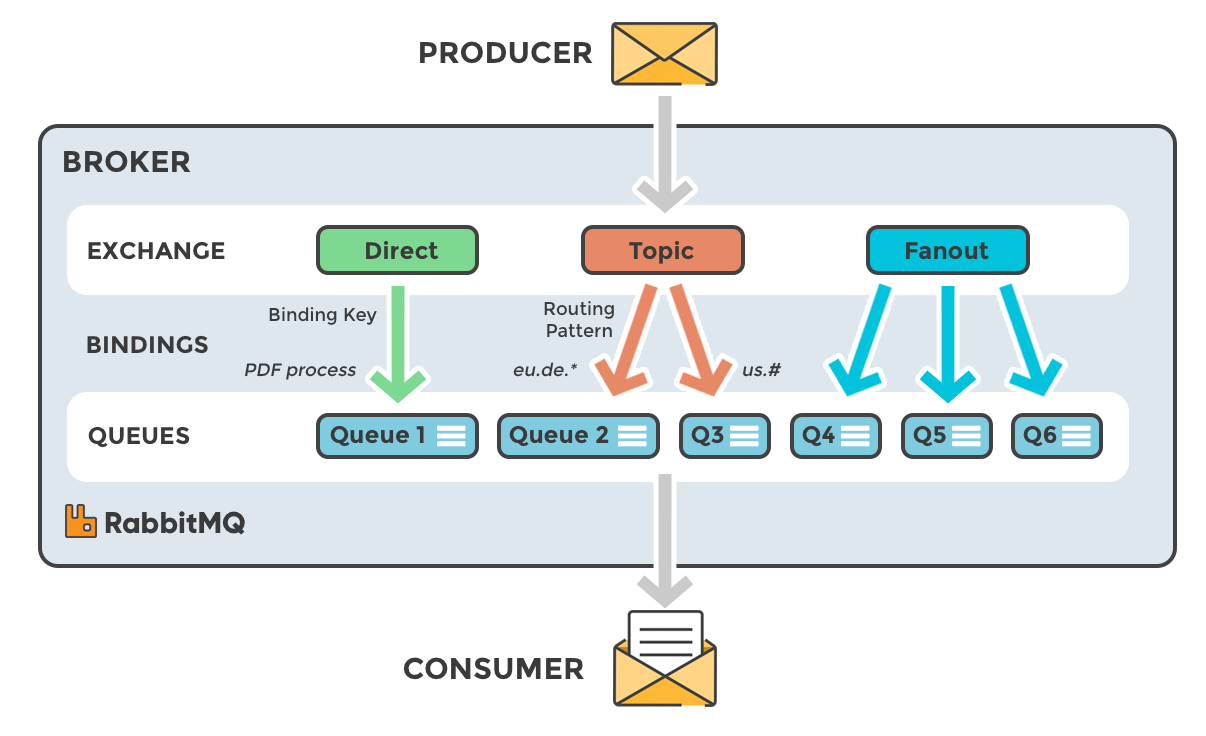
\includegraphics[width=0.8\textwidth]{Imagenes/Bitmap/rabbitmq}
    \caption{Ejemplo de los distintos tipos de exchange de RabbitMQ}
    \label{fig:rabbit}
\end{figure}

\begin{itemize}
    \item \textbf{Direct:} envía el mensaje solo a las colas que tienen una clave de enrutamiento (routing key) que coincide exactamente con la del mensaje.

    \item \textbf{Topic:} permite un enrutamiento más flexible usando patrones con comodines en la clave de enrutamiento. Útil para suscripciones parciales (ej., sensors.temperature.*).

    \item \textbf{Fanout:} reenvía el mensaje a todas las colas enlazadas, sin considerar la clave de enrutamiento. Ideal para difusiones o broadcasts.

    \item \textbf{Headers:} usa los campos del encabezado del mensaje en lugar de la clave de enrutamiento para decidir el destino.
\end{itemize}

Este sistema garantiza la entrega ordenada, confiable y asíncrona de los datos, siendo especialmente útil en arquitecturas orientadas a eventos donde los distintos componentes pueden fallar o estar temporalmente desconectados.

\subsection{WebSockets}

WebSocket es un protocolo de comunicación definido por el estándar RFC 6455~\citep{rfc6455_websocket} que permite establecer una conexión persistente y bidireccional entre un cliente (normalmente un navegador) y un servidor.


A diferencia del modelo HTTP tradicional basado en peticiones-respuestas, WebSocket permite que ambos extremos envíen datos en cualquier momento, lo que lo hace ideal para aplicaciones en tiempo real.
Una vez establecida la conexión, los datos se transmiten en forma de frames ligeros.

Gracias a esta arquitectura full-duplex, WebSocket es ampliamente utilizado en aplicaciones que requieran actualización inmediata sin recurrir a técnicas como polling.


